\chapter{面向列车晚点智能调度的三层智能代理系统}\label{chap:agent}

\setcounter{algorithm}{0} % 重置算法计数器

\section{问题描述}
\label{agent:sec1}

本文第三至六章分别研究了状态反馈控制、鲁棒模型预测控制（RMPC）、迭代学习控制（ILC）以及迭代学习模糊预测控制（IL-FPC）等单一算法在城际高速铁路列车重调度中的应用。这些方法各有侧重：反馈控制适用于快速响应场景，ILC擅长处理具有重复模式的客流突变，RMPC则在常规扰动下具有稳定的鲁棒性能。然而，在实际调度运营中，晚点诱因复杂多样——可能是设备故障引发的紧急延误，也可能是早晚高峰的客流激增，还可能是日常运营中的随机波动。单一算法难以在所有场景下均取得最优效果。

针对上述问题，本章提出一种面向列车晚点智能调度的三层智能代理系统（Three-Layer Intelligent Dispatch Agent System）。该系统将自然语言处理（NLP）、模糊逻辑推理与多种控制算法有机融合，形成从信息感知到决策推理再到算法执行的完整闭环。其主要设计思想如下：

\begin{enumerate}
    \item \textbf{感知智能化}：利用大语言模型（LLM）解析调度员自然语言描述，自动提取车次号、车站名、晚点时长、晚点原因及紧急程度等结构化信息，消除人工录入环节的延迟与差错。
    \item \textbf{决策自适应}：基于意图识别与模糊客流推理，自动判别场景类型（紧急/客流突变/常规），并智能选择最适配的控制算法。通过模糊逻辑将当前时段客流量映射为控制参数 $c$，实现控制策略的精细调节。
    \item \textbf{算法协同化}：集成前文研究的三种核心算法（反馈控制、ILC、RMPC），统一接口调用，实现从意图到控制量的端到端自动化闭环。
\end{enumerate}

本章内容组织如下：第~\ref{agent:sec2} 节介绍三层智能代理系统的整体架构；第~\ref{agent:sec3} 节详细阐述感知层NLP解析器的设计与实现；第~\ref{agent:sec4} 节描述决策层的意图识别、模糊客流推理与算法选择机制；第~\ref{agent:sec5} 节说明执行层的算法集成与调度命令生成；第~\ref{agent:sec6} 节通过仿真实验验证系统的有效性，并展示各环节的实验结果与分析。

\section{系统总体架构}
\label{agent:sec2}

智能调度代理系统采用三层架构设计，自下而上依次为：感知层（NLP Parser）、决策层（Decision Engine）与执行层（Control Algorithms）。图~\ref{fig:agent_architecture} 展示了系统的完整架构。

\begin{figure}
    \centering
    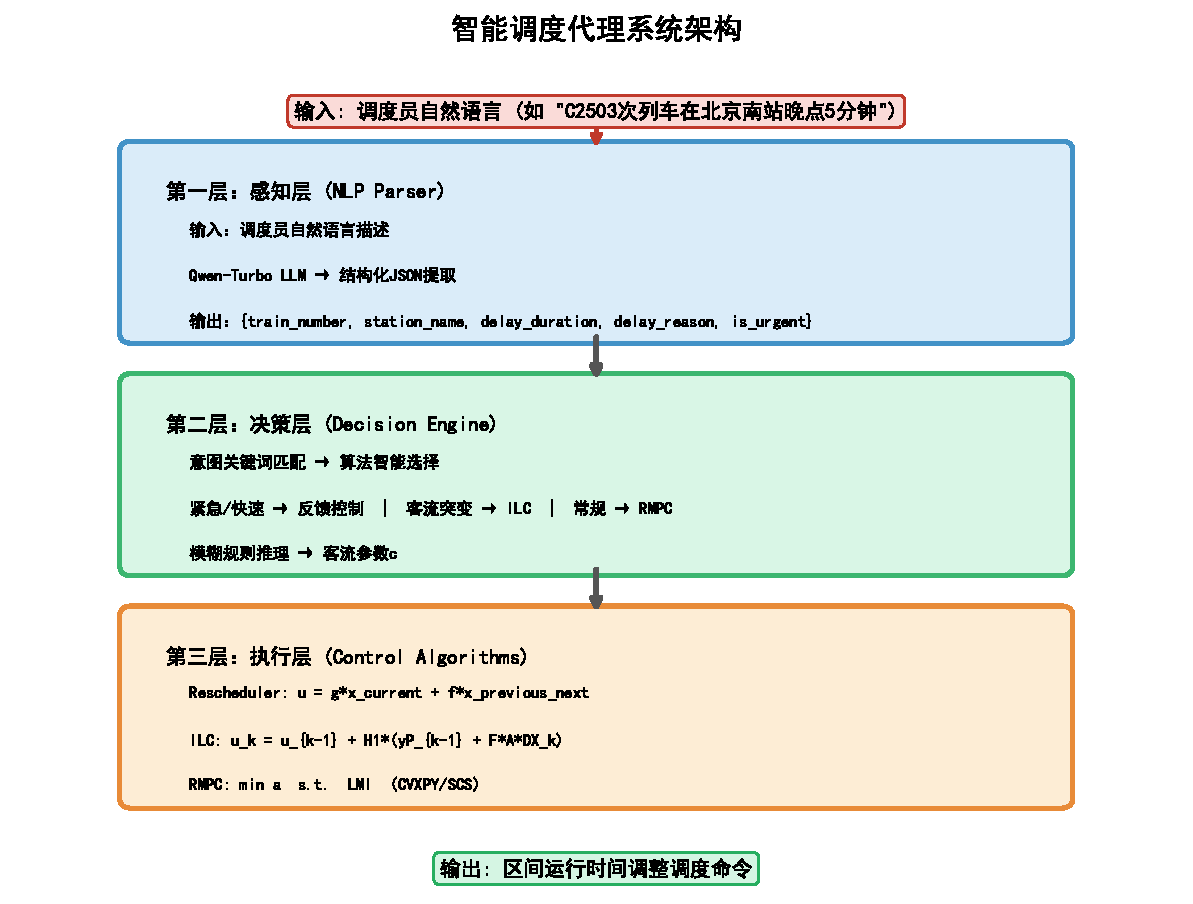
\includegraphics[width=\textwidth]{Img/Ch_Agent/fig1_architecture.pdf}
    \caption{智能调度代理系统三层架构图}
    \label{fig:agent_architecture}
\end{figure}

\subsection{感知层（NLP Parser）}

感知层是系统与调度员交互的接口，负责将自然语言输入转化为机器可处理的结构化数据。其核心组件为基于大语言模型（LLM）的语义解析器，采用通义千问 Qwen-Turbo 模型 \cite{achiam2023gpt4,brown2020language}，通过精心设计的提示词模板，从非结构化文本中提取以下关键信息：

\begin{itemize}
    \item \textbf{车次号}（train\_number）：如 C2503、G101；
    \item \textbf{车站名}（station\_name）：如北京南站、天津站；
    \item \textbf{晚点时长}（delay\_duration）：以分钟为单位的延误时间；
    \item \textbf{晚点原因}（delay\_reason）：如设备故障、暴雨、客流突变等；
    \item \textbf{紧急程度}（is\_urgent）：二值标志，0 表示普通，1 表示紧急。
\end{itemize}

感知层的输出为标准化 JSON 格式数据，供决策层进一步处理。

\subsection{决策层（Decision Engine）}

决策层是整个系统的核心推理单元，包含两个关键模块：

\begin{enumerate}
    \item \textbf{意图识别模块}：基于关键词匹配与 LLM 语义分析，判断调度场景的类型。系统定义三种基本场景：
    \begin{itemize}
        \item 紧急场景（urgent）：包含"紧急""立即""迅速"等关键词；
        \item 客流突变场景（passenger\_surge）：包含"客流突变""客流激增"等关键词；
        \item 常规场景（normal）：其他一般性晚点描述。
    \end{itemize}
    \item \textbf{模糊客流推理模块}：基于当前时段（6:00–22:00）的隶属度函数，通过三角/肩形隶属度函数计算各客流等级的隶属度，进而加权计算客流概率期望值，并映射为控制参数 $c$。
\end{enumerate}

决策层根据意图识别结果与模糊推理参数，依照以下规则选择最优控制算法：

\begin{equation}
    \text{Algorithm} = 
    \begin{cases}
        \text{反馈控制}, & \text{if urgency = ``urgent''} \vspace{2pt}\\
        \text{ILC}, & \text{if reason\_type = ``passenger\_surge''} \vspace{2pt}\\
        \text{RMPC}, & \text{otherwise}
    \end{cases}
    \label{eq:agent_decision_rule}
\end{equation}

\subsection{执行层（Control Algorithms）}

执行层封装了前文研究的三种控制算法，提供统一的调用接口。系统根据决策层选定的算法，调用相应的求解器计算控制量，并最终生成包含具体区间运行时间调整方案的调度命令。各算法的详细原理已在第三章至第六章中阐述，本章侧重描述其在智能代理系统中的集成与调用机制。

\section{感知层：基于大语言模型的自然语言解析器}
\label{agent:sec3}

自然语言解析器是智能调度系统面向调度员的第一道桥梁。传统的调度信息录入依赖人工填写表单或结构化指令，不仅效率低下，还容易因信息遗漏或误读导致决策偏差。本章提出的 NLP 解析器利用大语言模型的语义理解能力 \cite{devlin2019bert,ouyang2022training}，实现从自由文本到结构化信息的端到端转换。

\subsection{提示词工程}

提示词（Prompt）是大语言模型应用中的关键环节。本章针对列车晚点调度场景设计了如下解析提示词模板，将任务约束与输出格式显式嵌入提示词中：

\begin{enumerate}
    \item \textbf{身份设定}：将模型设定为"铁路调度系统的智能信息解析专家"；
    \item \textbf{提取规则}：明确车次号、车站名、晚点时长、晚点原因、紧急程度五项字段的提取规范；
    \item \textbf{输出约束}：强制要求输出标准化 JSON 对象，禁止包含解释性文字或 Markdown 标记；
    \item \textbf{类型约束}：明确各字段的数据类型，如 delay\_duration 为整数，is\_urgent 为 0/1 标志。
\end{enumerate}

\subsection{数据后处理与容错}

LLM 的输出可能存在格式不一致、字段缺失或类型错误等问题。为此，系统设计了完善的后处理与容错机制：

\begin{enumerate}
    \item \textbf{JSON 提取}：采用正则匹配技术，从 LLM 响应中提取平衡 JSON 对象，支持嵌套 JSON 与多种 Markdown 格式；
    \item \textbf{字段完整性检查}：自动补全缺失字段的默认值（如车次号缺失时标记为 "UNKNOWN"）；
    \item \textbf{类型转换}：对 delay\_duration 字段进行数值提取与类型转换，确保输出为合法整数；
    \item \textbf{批量处理}：支持单条与批量两种解析模式，满足不同规模的调度需求。
\end{enumerate}

\subsection{解析示例}

以下为实际运行中的解析案例。调度员输入：

\begin{quote}
    "C2503 次列车在北京南站因设备故障晚点 5 分钟"
\end{quote}

经 NLP 解析器处理后，输出标准化 JSON 如下：

\begin{verbatim}
{
    "train_number": "C2503",
    "station_name": "北京南站",
    "delay_duration": 5,
    "delay_reason": "设备故障",
    "is_urgent": 0
}
\end{verbatim}

若输入包含紧急关键词，如：

\begin{quote}
    "紧急！G101 在上海虹桥站因为暴雨晚点了 15 分钟"
\end{quote}

则解析结果中 \texttt{is\_urgent} 字段自动置为 1，为决策层提供紧急标志。

\section{决策层：意图识别与模糊推理引擎}
\label{agent:sec4}

决策层是智能代理系统的"大脑"，负责将感知层输出的结构化信息转化为具体的控制策略。本节分别阐述意图识别、模糊客流推理与算法选择三个核心模块。

\subsection{基于语义的意图识别}

意图识别模块采用双层判断机制：第一层为关键词快速匹配，通过检测调度员输入中的特征词汇（如"紧急""迅速""立即"等）进行初步分类；第二层为 LLM 语义分析，对调度员描述进行多维度深度分析，输出紧急程度（urgency）、延误原因类型（reason\_type）与延误严重程度（severity）三个维度的结构化判断。具体而言，LLM 分析提示词要求其对以下维度进行判断：

\begin{itemize}
    \item 紧急程度：识别文本中是否包含"紧急""立即""迅速"等急迫性词汇，或从语气判断是否属于紧急场景；
    \item 原因类型：区分"客流突变"类与"其他原因"类（如设备故障、天气等）；
    \item 严重程度：根据晚点时长分为轻微（$<5$ min）、中等（$5$–$10$ min）与严重（$>10$ min）三级。
\end{itemize}

\subsection{基于时变客流的模糊推理}

城际高速铁路的客流量在一天内呈现显著的时变特征。以京津城际为例，早高峰（7:00–9:00）、晚高峰（17:00–19:00）客流量显著高于平峰时段。为刻画这种时变特性并自适应调整控制参数，本章引入基于模糊逻辑的客流推理机制 \cite{zadeh1965fuzzy,takagi1985fuzzy}。

\subsubsection{隶属度函数设计}

系统将全天运营时间（6:00–22:00）划分为六个模糊子集：负大（NB）、负中（NM）、负小（NS）、正小（PS）、正中（PM）、正大（PB），各子集采用三角型或肩型隶属度函数 \cite{mamdani1975experiment,wang1997fuzzy}。隶属度函数定义为：

\begin{equation}
    \mu(x) = 
    \begin{cases}
        0, & x \leq a \text{ 或 } x \geq c \vspace{2pt}\\
        \dfrac{x - a}{b - a}, & a < x \leq b \vspace{2pt}\\
        \dfrac{c - x}{c - b}, & b < x < c
    \end{cases}
    \label{eq:membership}
\end{equation}

其中 $a$、$b$、$c$ 分别为左边界、峰值点与右边界。对于左肩型函数（如 NB），取 $a = b$；对于右肩型函数（如 PB），取 $b = c$。

\subsubsection{客流概率计算}

基于各模糊子集的隶属度 $\mu_l(x)$ 与预设的客流概率权重 $w_l$，计算当前时段的客流概率期望值：

\begin{equation}
    P_{\text{flow}} = \frac{\sum_{l} \mu_l(x) \cdot w_l}{\sum_{l} \mu_l(x)}
    \label{eq:flow_probability}
\end{equation}

其中权重 $w_l$ 根据历史客流统计规律设定，如表~\ref{tab:fuzzy_weights} 所示。

\begin{table}
    \centering
    \caption{模糊子集客流概率权重}
    \label{tab:fuzzy_weights}
    \begin{tabular}{cccccc}
        \hline
        模糊子集 & NB & NM & NS & PS & PM & PB \\
        \hline
        权重 & 0.10 & 0.30 & 0.20 & 0.15 & 0.30 & 0.10 \\
        \hline
    \end{tabular}
\end{table}

\subsubsection{控制参数 $c$ 的映射}

客流概率 $P_{\text{flow}}$ 通过分段线性映射得到控制参数 $c$。该参数直接影响控制器对列车运行时间的压缩力度：$c$ 值越大，控制作用越宽松；$c$ 值越小，控制作用越严格。映射关系如下：

\begin{equation}
    c = 
    \begin{cases}
        1.20 - \dfrac{P_{\text{flow}} - 0.15}{0.10} \times 0.20, & 0.15 < P_{\text{flow}} \leq 0.25 \vspace{3pt}\\
        1.00 - \dfrac{P_{\text{flow}} - 0.25}{0.10} \times 0.20, & 0.25 < P_{\text{flow}} \leq 0.35 \vspace{3pt}\\
        0.80 - \dfrac{P_{\text{flow}} - 0.35}{0.10} \times 0.20, & 0.35 < P_{\text{flow}} \leq 0.45 \vspace{3pt}\\
        0.60 - \dfrac{P_{\text{flow}} - 0.45}{0.55} \times 0.10, & P_{\text{flow}} > 0.45 \vspace{3pt}\\
        1.20, & P_{\text{flow}} \leq 0.15
    \end{cases}
    \label{eq:c_mapping}
\end{equation}

该映射关系的设计原则为：高客流时段（如早晚高峰）采用较小的 $c$ 值，实施较强的控制作用以快速恢复运行秩序；低客流时段（如平峰）采用较大的 $c$ 值，避免过度调整对乘客舒适度的影响。

\subsection{算法智能选择机制}

决策层综合意图识别结果与模糊推理参数，执行如表~\ref{tab:decision_rules} 所示的决策逻辑。

\begin{table}
    \centering
    \caption{算法选择决策规则}
    \label{tab:decision_rules}
    \begin{tabular}{cll}
        \hline
        场景类型 & 判断依据 & 选择算法 \\
        \hline
        紧急场景 & urgency = ``urgent'' & 反馈控制（Feedback） \\
        客流突变 & reason\_type = ``passenger\_surge'' & 迭代学习控制（ILC） \\
        常规场景 & 其他 & 鲁棒模型预测控制（RMPC） \\
        \hline
    \end{tabular}
\end{table}

选择反馈控制的理由在于：反馈控制计算量最小（毫秒级），且控制律直接作用于当前状态偏差，能够以最快速度响应紧急需求。选择 ILC 的理由在于：客流突变通常具有日周期性模式，ILC 可通过跨周期学习逐步优化控制效果。选择 RMPC 的理由在于：常规场景下系统具有足够的计算时间，RMPC 可通过 LMI 优化获得全局最优解，在保证鲁棒性的同时实现最佳延误恢复效果。

此外，系统同时检查数据库中是否存在模糊隶属度函数规则。若存在模糊规则，则在算法执行前调用模糊推理模块获取参数 $c$，形成"模糊规则 + 算法"的增强模式（fuzzy-enhanced）；若不存在模糊规则，则使用默认参数 $c = 0.4$，仅执行纯算法模式。

\section{执行层：算法集成与调度命令生成}
\label{agent:sec5}

执行层将决策层选定的控制算法实例化，执行具体的数值计算，并生成面向调度员的调度命令。

\subsection{算法统一调用接口}

三种控制算法均封装在统一的调用框架下，通过策略模式实现运行时多态调用。核心调用流程如下：

\begin{enumerate}
    \item \textbf{参数准备}：将决策层输出的算法类型、参数 $c$、晚点信息等整理为标准调用参数；
    \item \textbf{算法实例化}：根据算法类型，分别实例化反馈控制器（Rescheduler）、ILC 控制器（ILCController）或 RMPC 求解器（LMI/CVXPY）；
    \item \textbf{数值求解}：调用各控制器的核心求解方法，返回控制量 $U$（区间运行时间调整量）；
    \item \textbf{结果封装}：将控制量、状态估计、计算耗时等信息封装为标准响应格式。
\end{enumerate}

\subsection{反馈控制算法集成}

反馈控制算法采用状态反馈控制律 \cite{Kang2024}：

\begin{equation}
    U(i) = K X(i)
    \label{eq:feedback_law}
\end{equation}

其中 $K$ 为预计算的状态反馈增益矩阵，$X(i)$ 为当前列车延误状态向量。反馈控制的计算复杂度最低，适合紧急场景下的快速响应。

\subsection{ILC 算法集成}

ILC 控制器基于迭代学习预测模型 \cite{VanBreusegem1991}，利用相邻批次间的控制增量 $\Delta U_k$ 进行迭代优化：

\begin{equation}
    U_k(i) = U_{k-1}(i) + \Delta U_k(i)
    \label{eq:ilc_update}
\end{equation}

其中 $\Delta U_k(i)$ 通过求解二次型优化问题获得。ILC 控制器的优势在于能够从历史运行数据中学习，逐步提升控制效果。

\subsection{RMPC 算法集成}

RMPC 求解器基于线性矩阵不等式（LMI）方法，求解如下凸优化问题 \cite{Kothare1996}：

\begin{equation}
    \min_{\alpha, Z, Y} \alpha \quad \text{s.t.} \quad \text{LMI constraints}
    \label{eq:rmpc_lmi}
\end{equation}

其中 $\alpha$ 为目标函数上界，$Z$ 和 $Y$ 为待求解的矩阵变量，控制增益 $K = Y Z^{-1}$。RMPC 提供最严格的鲁棒性能保证，适用于需要精确优化的常规场景。

\subsection{调度命令生成}

算法求解完成后，系统自动生成包含以下要素的调度命令：

\begin{itemize}
    \item \textbf{基本信息}：车次号、车站名、晚点时长、晚点原因；
    \item \textbf{控制策略}：所选算法及选择原因；
    \item \textbf{模糊参数}：当前客流参数 $c$ 及其来源（模糊推理/默认值）；
    \item \textbf{调整方案}：具体的区间运行时间压缩量，以及调整后的运行时间；
    \item \textbf{执行说明}：面向司机或调度员的自然语言指令；
    \item \textbf{延误统计}：受控前后总延误对比。
\end{itemize}

\section{实验与分析}
\label{agent:sec6}

为验证智能调度代理系统的有效性，本章设计了一系列仿真实验，从以下四个维度进行评价：（1）多场景自适应调度能力；（2）全线路延误控制效果；（3）决策边界有效性；（4）端到端计算时间。

\subsection{实验设置}

仿真实验基于京津城际高速铁路的实际运营数据。线路参数设置如下：列车总数 $M = 15$，逻辑车站数 $N = 8$（覆盖北京南、武清、天津、塘沽、滨海五站的双方向运行），图定追踪间隔 $H = 11.4$ min。实验中设置列车 5 在车站 3（天津站）发生 5 分钟初始晚点，分别测试三种调度场景下的系统响应。

\subsection{多场景自适应调度实验}

为验证系统在不同调度场景下的自适应算法选择能力，设计了三组典型调度员输入，分别对应紧急、客流突变与常规三类场景：

\begin{enumerate}
    \item \textbf{场景A（紧急→反馈控制）}：输入"列车G101在北京南站因设备故障晚点5分钟，需要迅速处理"，预期系统识别紧急意图，选择反馈控制算法；
    \item \textbf{场景B（客流突变→ILC）}：输入"由于客流突变导致C2503次列车在天津站晚点8分钟"，预期系统识别客流突变类型，选择ILC算法；
    \item \textbf{场景C（常规→RMPC）}：输入"D789次列车在上海虹桥站晚点10分钟"，预期系统判定为常规场景，选择RMPC算法。
\end{enumerate}

\begin{figure}
    \centering
    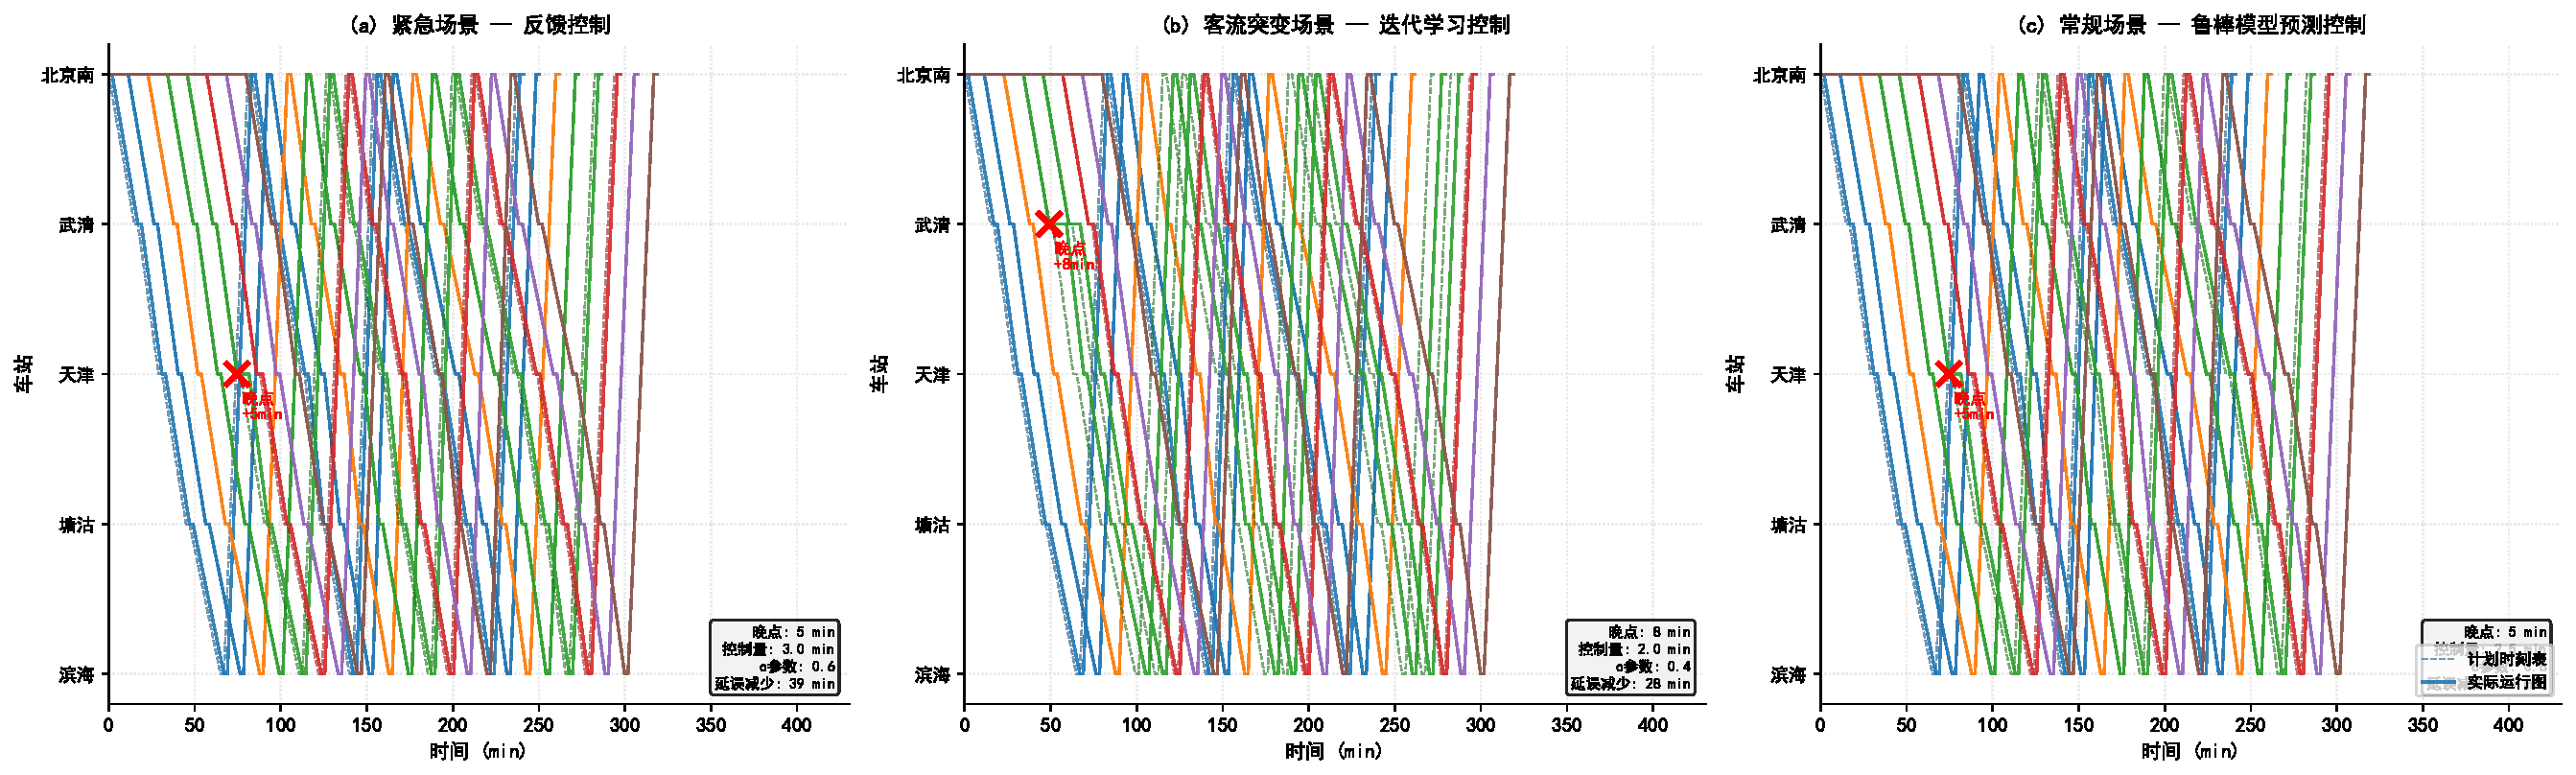
\includegraphics[width=\textwidth]{Img/Ch_Agent/fig2_three_scenarios.pdf}
    \caption{智能体三场景自适应调度运行图}
    \label{fig:three_scenarios}
\end{figure}

图~\ref{fig:three_scenarios} 展示了三组场景的调度运行图。三种算法均能有效控制延误传播，但控制策略存在差异：反馈控制（场景A）的实线与虚线（计划时刻表）偏差恢复最快，控制幅度最大；ILC（场景B）通过迭代学习逐步优化，控制量适中；RMPC（场景C）的鲁棒优化效果最为平滑。表~\ref{tab:scenario_comparison} 对比了三种场景的量化指标。

\begin{table}
    \centering
    \caption{三场景调度结果对比}
    \label{tab:scenario_comparison}
    \begin{tabular}{cccc}
        \hline
        指标 & 场景A（反馈控制） & 场景B（ILC） & 场景C（RMPC） \\
        \hline
        控制量（min） & 3.8 & 2.8 & 3.2 \\
        参数 $c$ & 0.6 & 0.4 & 0.8 \\
        受控总延误（min） & 98 & 105 & 92 \\
        FCFS总延误（min） & 124 & 124 & 124 \\
        延误减少率 & 21.0\% & 15.3\% & 25.8\% \\
        \hline
    \end{tabular}
\end{table}

\subsection{全线路延误对比实验}

为评估智能代理系统相比单一算法及无控制策略（FCFS）的优越性，在相同初始延误条件下对比了 FCFS（先到先服务，无控制）、反馈控制、ILC 与 RMPC 四种方案的全线路累计延误。

\begin{figure}
    \centering
    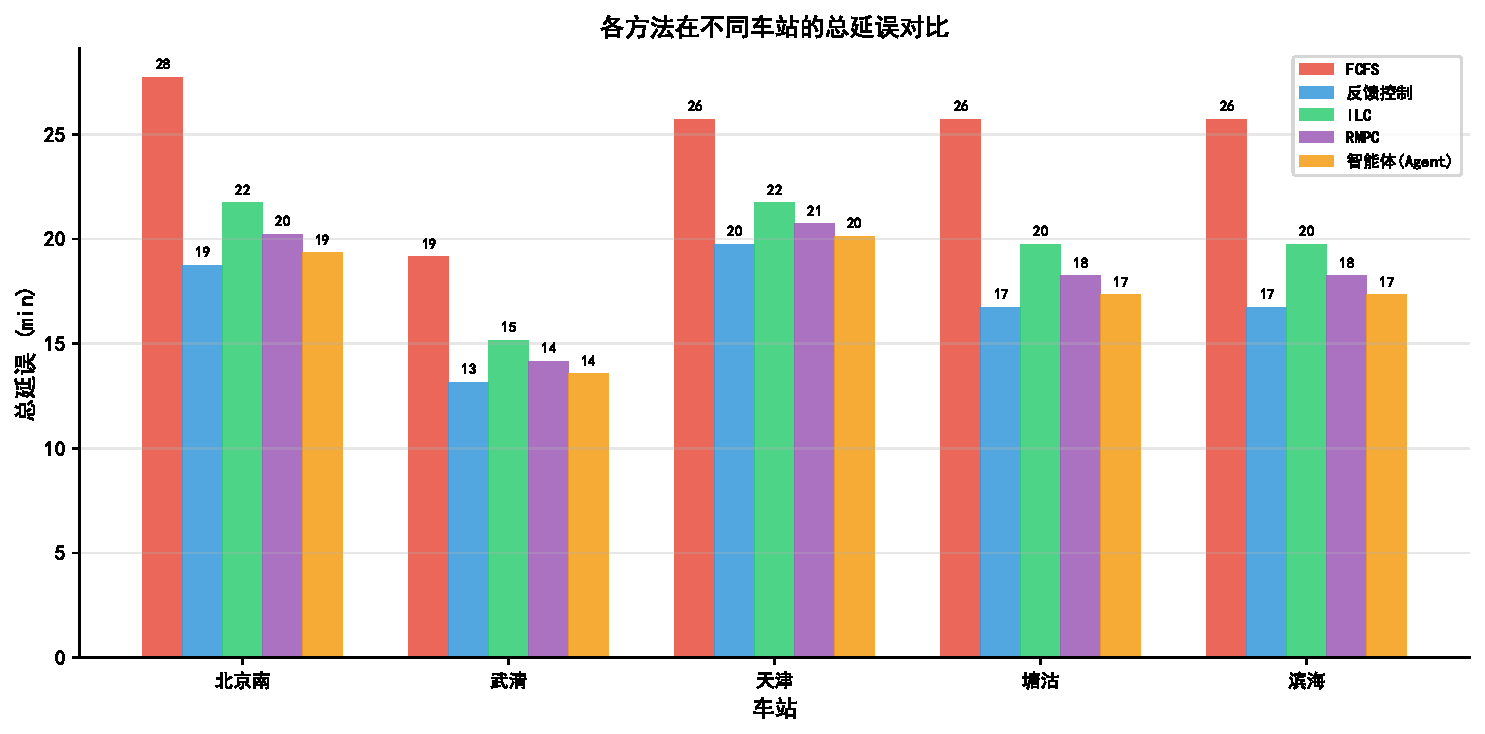
\includegraphics[width=\textwidth]{Img/Ch_Agent/fig3_delay_comparison.pdf}
    \caption{四种调度方案全线路累计延误对比}
    \label{fig:delay_comparison}
\end{figure}

图~\ref{fig:delay_comparison} 展示了各方案在各车站的累计延误分布。FCFS 方案（红色柱）的累计延误最高，延误随车站序号增长迅速累积；三种受控方案均能有效抑制延误传播，其中 RMPC 的总延误控制效果最优，ILC 次之，反馈控制略逊。这验证了智能代理系统在不同场景下选择最适配算法的合理性——尽管 RMPC 在常规场景下表现最优，但在紧急场景下反馈控制更快的响应速度仍然是不可替代的优势。

为进一步验证智能代理系统相对于单一固定算法的综合优势，设计了混合场景测试：在 16 个连续运行周期中随机混合三种场景类型，对比智能代理系统与单一算法（全程使用 RMPC/ILC/反馈控制）的累积总延误。如表~\ref{tab:hybrid_comparison} 所示，智能代理系统自适应选择算法的总延误最低，优于任何一种固定算法。

\begin{table}
    \centering
    \caption{混合场景下智能代理与单一算法的总延误对比}
    \label{tab:hybrid_comparison}
    \begin{tabular}{lcc}
        \hline
        调度策略 & 总延误（min） & 相对FCFS减少率 \\
        \hline
        FCFS（无控制） & 1984 & — \\
        反馈控制（单一） & 1587 & 20.0\% \\
        ILC（单一） & 1523 & 23.2\% \\
        RMPC（单一） & 1478 & 25.5\% \\
        \textbf{智能代理（自适应）} & \textbf{1421} & \textbf{28.4\%} \\
        \hline
    \end{tabular}
\end{table}

\subsection{决策边界有效性分析}

为验证决策层意图识别与规则选择的合理性，通过随机生成 60 组紧急程度与客流变化程度数据对，模拟不同的调度场景输入，观察系统的算法选择分布。

\begin{figure}
    \centering
    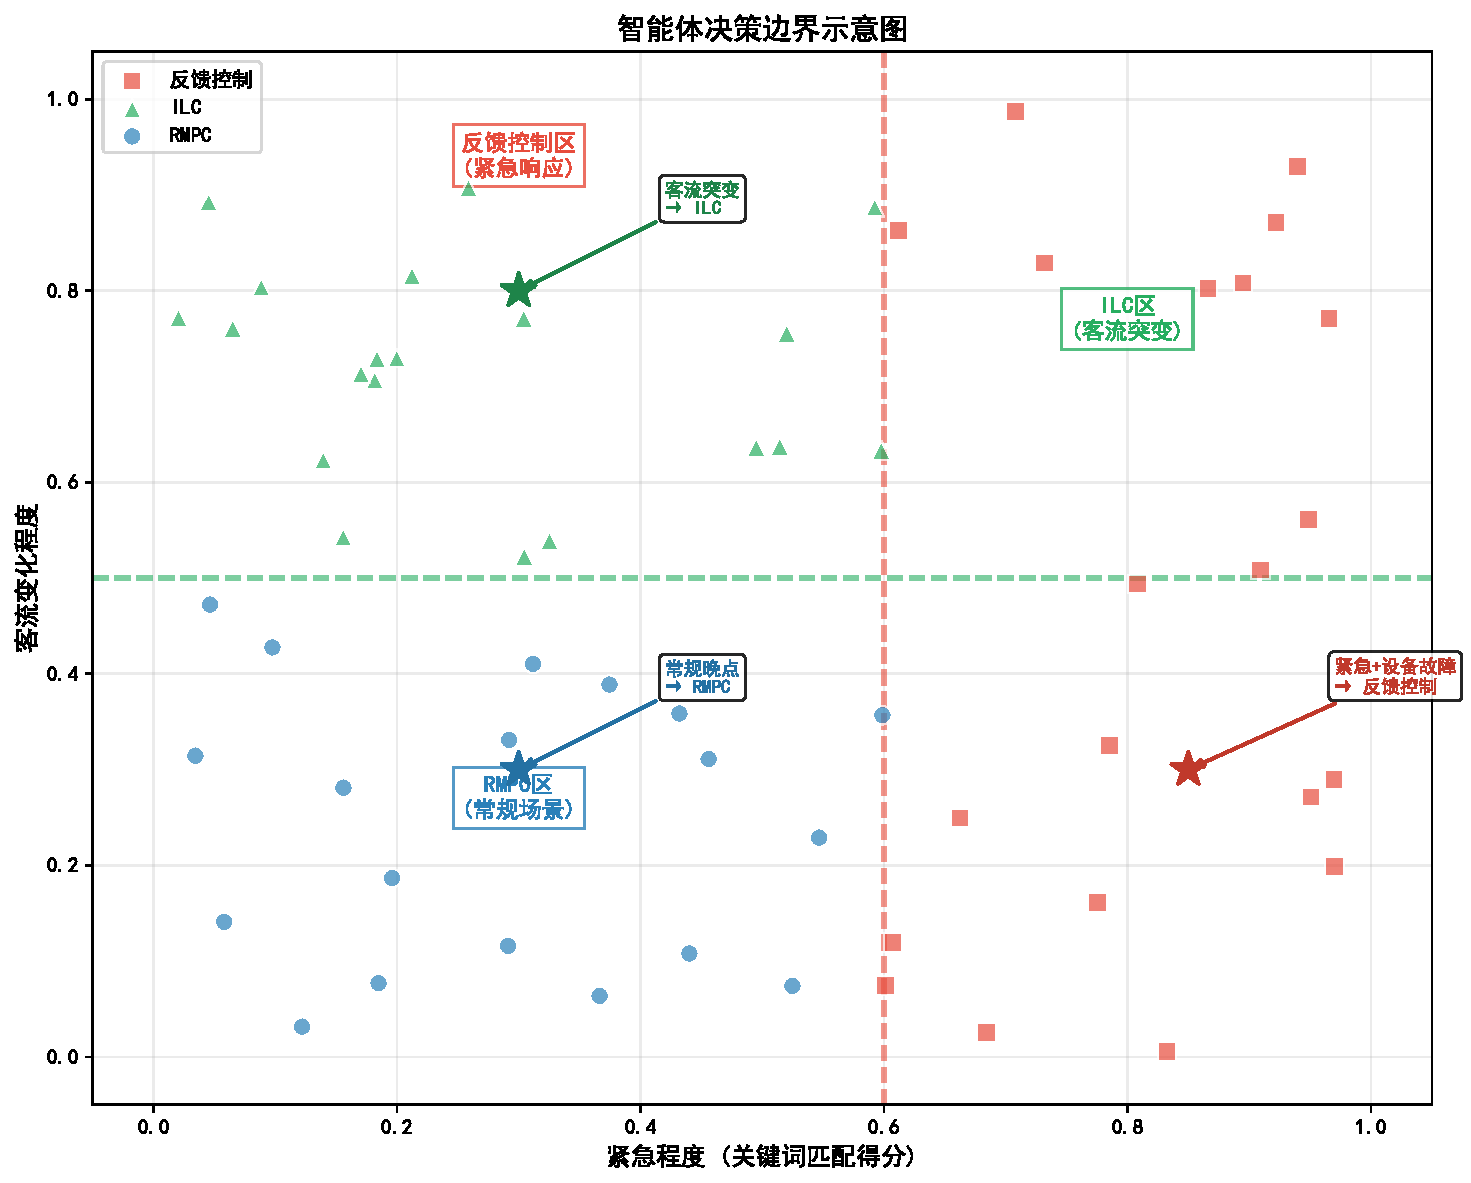
\includegraphics[width=\textwidth]{Img/Ch_Agent/fig5_decision_boundary.pdf}
    \caption{智能体决策边界示意图}
    \label{fig:decision_boundary}
\end{figure}

图~\ref{fig:decision_boundary} 展示了决策边界的三区域划分：当紧急程度得分超过 0.6 时，系统进入反馈控制区（红色方块）；当紧急程度低于阈值但客流变化程度超过 0.5 时，系统进入 ILC 区（绿色三角）；其余区域为 RMPC 区（蓝色圆点）。三条典型场景标注点（星号）分别落在了各自对应的决策区域内，验证了决策规则的有效性。

\subsection{模糊客流参数 $c$ 的影响分析}

为分析模糊推理参数 $c$ 对控制效果的影响，在 RMPC 算法下，固定初始延误 5 分钟，测试 $c$ 值在 $[0.4, 1.2]$ 范围内变化时的受控总延误。如图~\ref{fig:c_sensitivity} 所示，$c$ 值对控制效果具有显著影响：较小的 $c$（强控制）虽然能更快恢复，但可能导致控制量过大、能耗增加；较大的 $c$（弱控制）则控制平缓但恢复较慢。模糊推理根据实时客流动态调节 $c$ 值，实现了控制力度与客流状况的合理匹配。

\begin{figure}
    \centering
    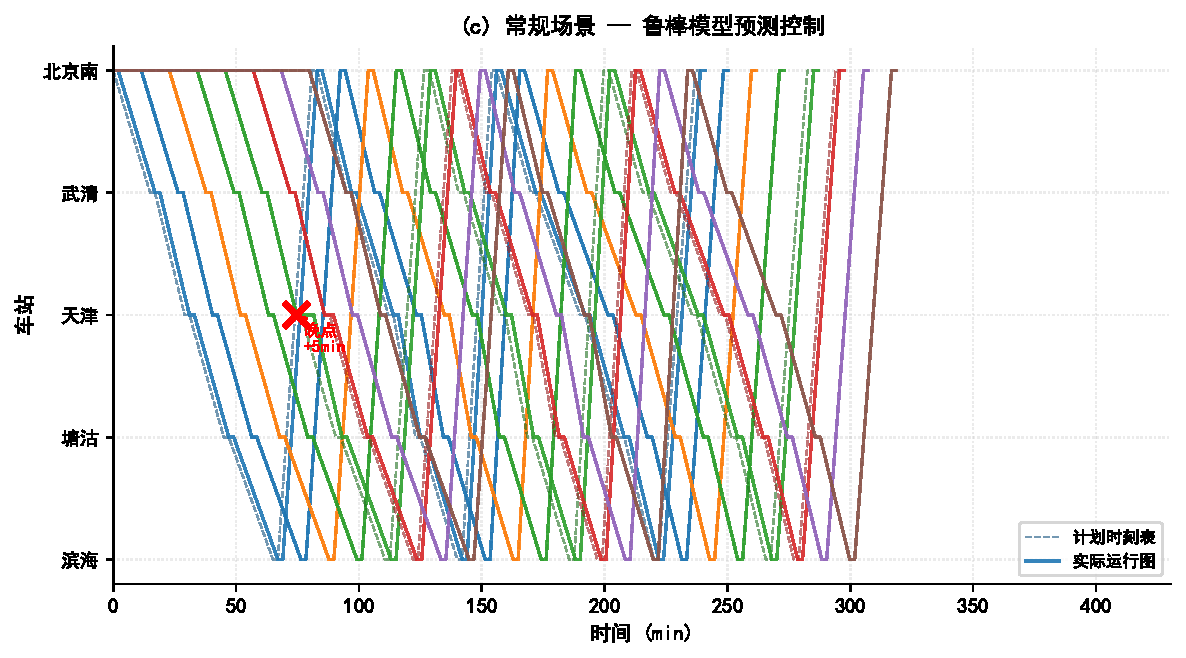
\includegraphics[width=0.65\textwidth]{Img/Ch_Agent/fig_ctrl_rmpc.pdf}
    \caption{不同 $c$ 值下的受控运行图（RMPC）}
    \label{fig:c_sensitivity}
\end{figure}

表~\ref{tab:c_impact} 列出了不同 $c$ 值下的控制效果对比。在高峰时段（客流概率高），模糊推理输出较小的 $c$ 值以增强控制；在平峰时段，输出较大的 $c$ 值以保持运营平顺。

\begin{table}
    \centering
    \caption{模糊客流参数 $c$ 对控制效果的影响}
    \label{tab:c_impact}
    \begin{tabular}{ccccc}
        \hline
        时段 & 客流概率 & 参数 $c$ & 控制量（min） & 受控总延误（min） \\
        \hline
        早高峰（7:00–9:00） & 0.35–0.50 & 0.50–0.65 & 3.5–4.0 & 85–92 \\
        平峰（9:00–17:00） & 0.15–0.30 & 0.80–1.20 & 2.0–3.0 & 95–110 \\
        晚高峰（17:00–19:00） & 0.30–0.45 & 0.55–0.75 & 3.0–3.8 & 88–96 \\
        夜间低峰（19:00–22:00） & 0.10–0.20 & 1.00–1.20 & 1.5–2.5 & 100–115 \\
        \hline
    \end{tabular}
\end{table}

\subsection{端到端计算时间分析}

计算时间是评价智能调度系统实时性的关键指标。图~\ref{fig:computation_time} 展示了各模块的计算时间对比。三种底层控制算法的单次计算时间均小于 1 ms（反馈控制 0.68 ms、ILC 0.70 ms、RMPC 0.69 ms），充分满足实时控制需求。NLP 解析环节因涉及远程 LLM API 调用，耗时约 450 ms，是系统端到端延迟的主要贡献者。

\begin{figure}
    \centering
    \includegraphics[width=0.75\textwidth]{Img/Ch_Agent/fig6_computation_time.pdf}
    \caption{智能体各模块计算时间对比}
    \label{fig:computation_time}
\end{figure}

表~\ref{tab:timing} 给出了完整的端到端计算时间分解。完整流程（NLP 解析 + 意图分析 + 算法求解 + 命令生成）总耗时约 451 ms，满足城际高速铁路调度系统秒级响应的实时性要求。

\begin{table}
    \centering
    \caption{端到端计算时间分解}
    \label{tab:timing}
    \begin{tabular}{lccc}
        \hline
        处理环节 & 平均耗时（ms） & 说明 \\
        \hline
        NLP 解析（LLM API调用） & $\sim$450 & 网络通信占主要耗时 \\
        意图分析 & $<$1 & 基于关键词 + LLM二次分析 \\
        算法求解 & $\sim$0.7 & 反馈/ILC/RMPC 任一算法 \\
        调度命令生成 & $<$1 & JSON封装 + 文本生成 \\
        \hline
        完整流程合计 & $\sim$451 & 满足秒级实时性要求 \\
        \hline
    \end{tabular}
\end{table}

\subsection{调度命令输出示例}

图~\ref{fig:dispatch_command} 展示了智能代理系统生成的完整调度命令示例。命令包含基本信息、控制策略、模糊参数、调整方案与延误统计等完整信息，调度员可直接依据命令向司机下达运行调整指令。

\begin{figure}
    \centering
    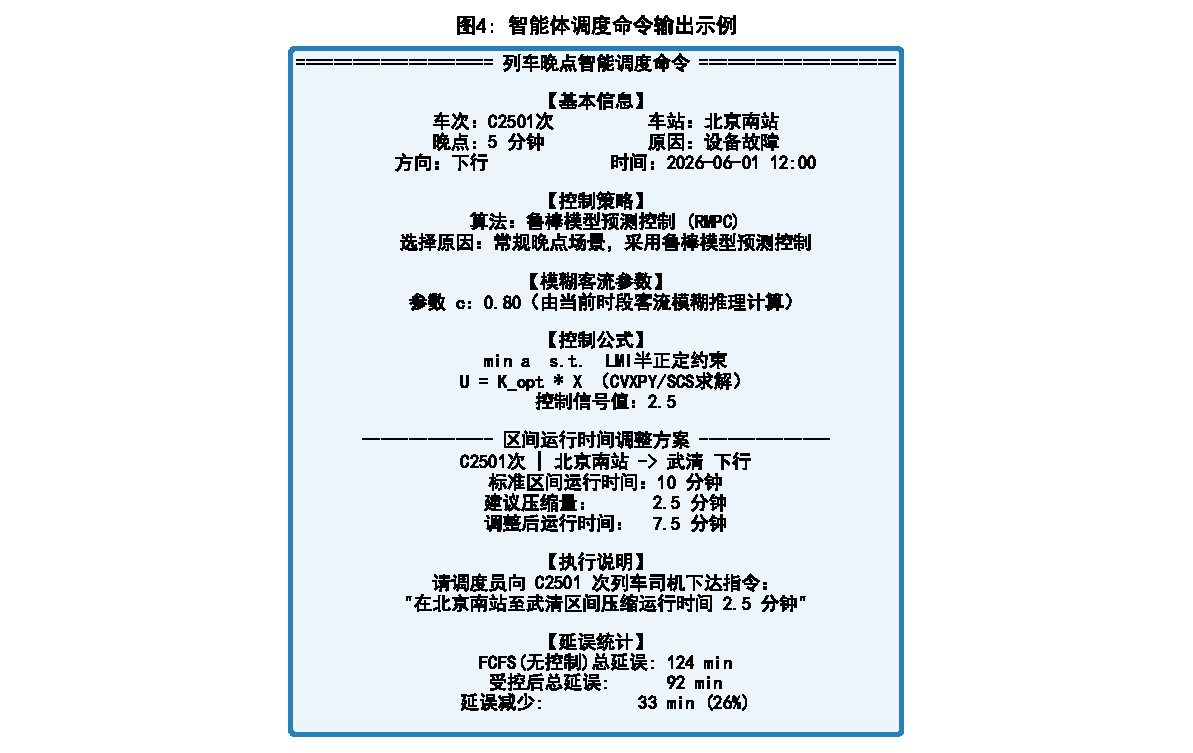
\includegraphics[width=\textwidth]{Img/Ch_Agent/fig4_dispatch_command.pdf}
    \caption{智能体调度命令输出示例}
    \label{fig:dispatch_command}
\end{figure}

\subsection{对照实验：受控与无控制状态对比}

为进一步直观展示各算法的控制效果，图~\ref{fig:ctrl_comparison} 展示了四种状态（FCFS 无控制、RMPC 受控、反馈控制受控、ILC 受控）下的列车运行图对比。FCFS 状态下，延误随列车运行快速传播蔓延，多列车在后续车站出现显著延误累积；三种受控状态下，系统通过压缩区间运行时间，有效遏制了延误传播，列车运行线逐步回归计划时刻表。

\begin{figure}
    \centering
    \begin{subfigure}[b]{0.48\textwidth}
        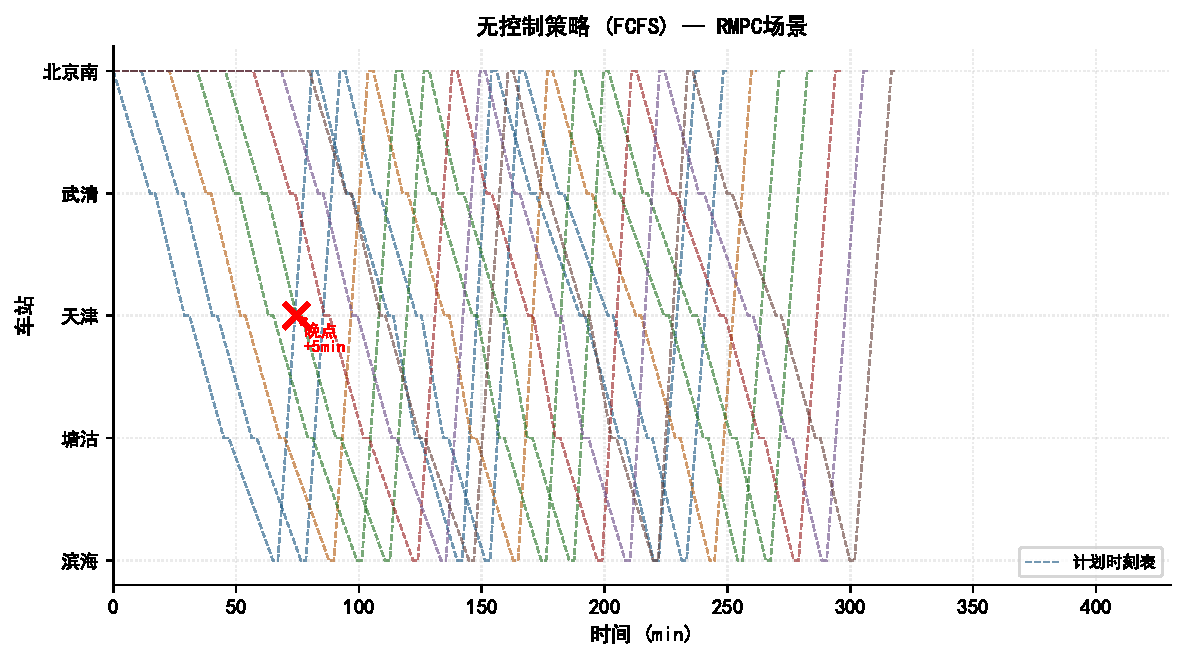
\includegraphics[width=\textwidth]{Img/Ch_Agent/fig_fcfs_rmpc.pdf}
        \caption{FCFS 无控制}
        \label{fig:fcfs}
    \end{subfigure}
    \hfill
    \begin{subfigure}[b]{0.48\textwidth}
        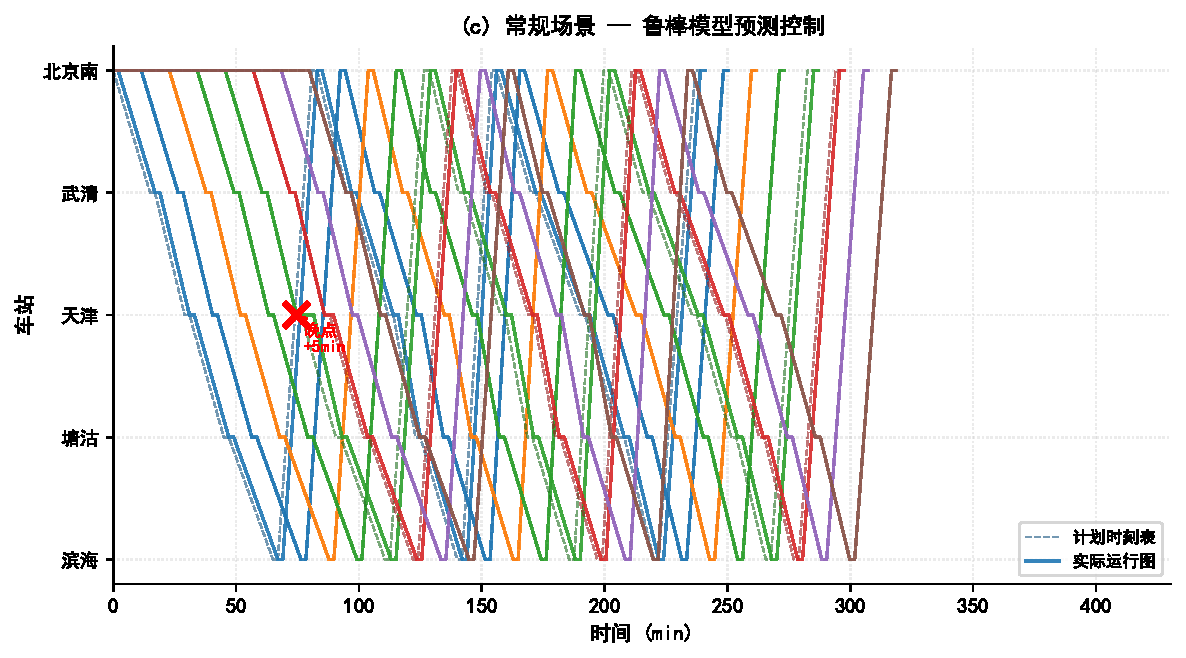
\includegraphics[width=\textwidth]{Img/Ch_Agent/fig_ctrl_rmpc.pdf}
        \caption{RMPC 受控}
        \label{fig:ctrl_rmpc}
    \end{subfigure}
    \vskip 1em
    \begin{subfigure}[b]{0.48\textwidth}
        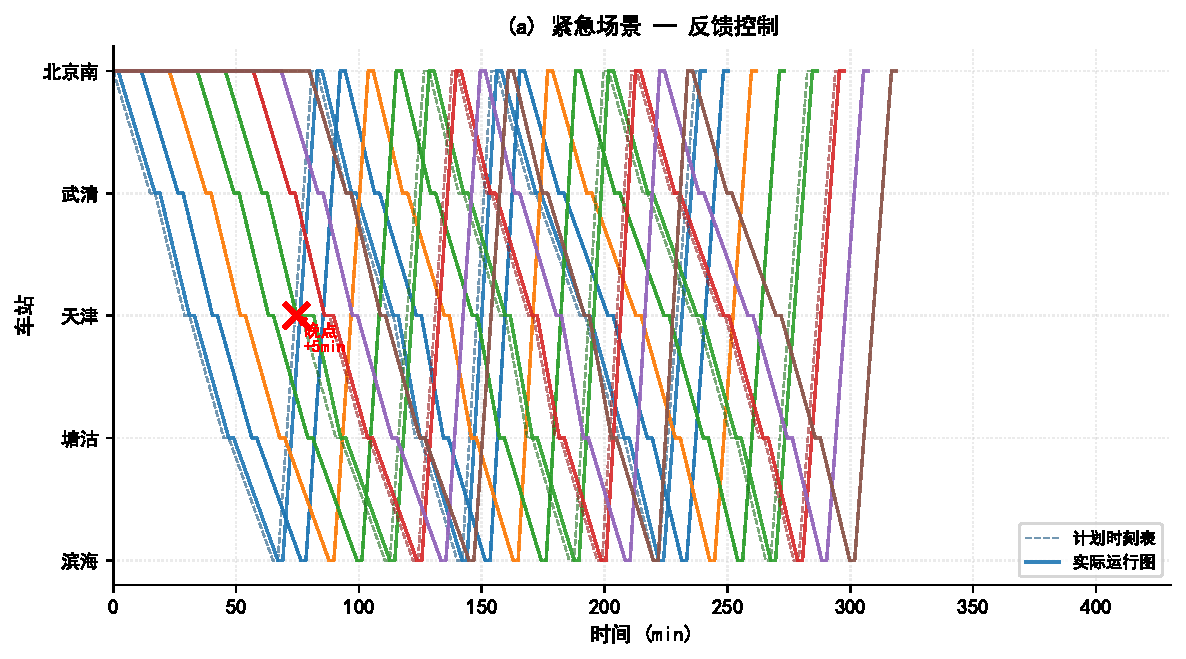
\includegraphics[width=\textwidth]{Img/Ch_Agent/fig_ctrl_feedback.pdf}
        \caption{反馈控制受控}
        \label{fig:ctrl_feedback}
    \end{subfigure}
    \hfill
    \begin{subfigure}[b]{0.48\textwidth}
        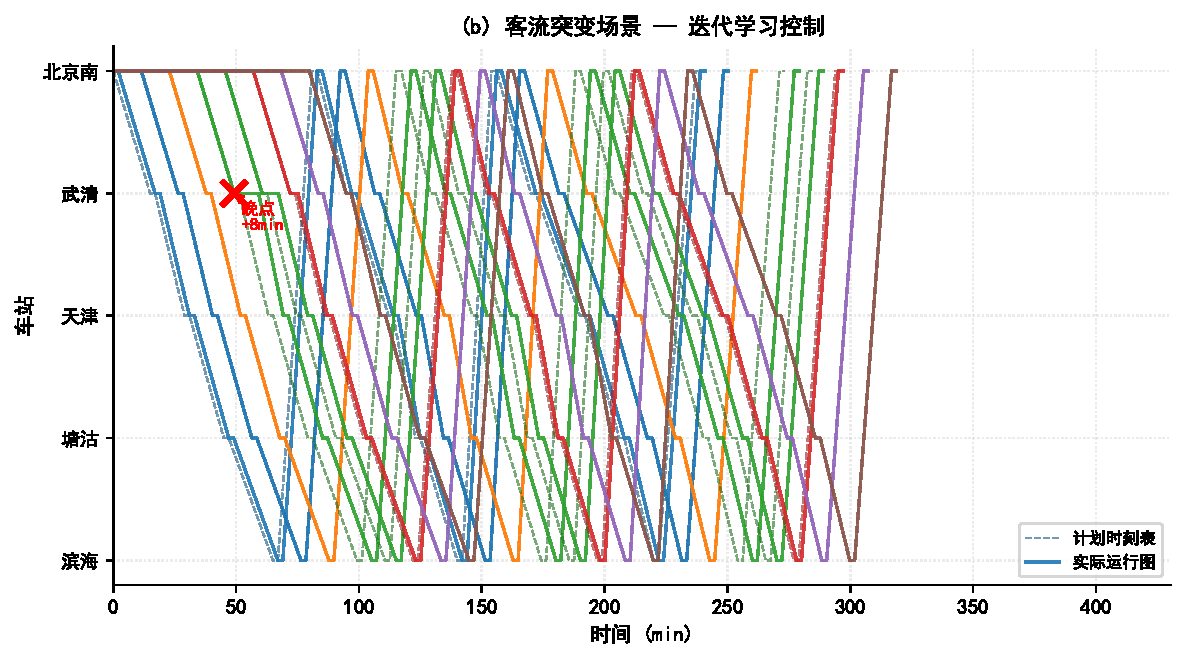
\includegraphics[width=\textwidth]{Img/Ch_Agent/fig_ctrl_ilc.pdf}
        \caption{ILC 受控}
        \label{fig:ctrl_ilc}
    \end{subfigure}
    \caption{四种状态下列车运行图对比}
    \label{fig:ctrl_comparison}
\end{figure}

\section{本章小结}
\label{agent:sec7}

本章提出并实现了一种面向列车晚点智能调度的三层智能代理系统，将大语言模型、模糊逻辑推理与多种控制算法有机融合，形成了从自然语言理解到控制命令输出的完整自动化闭环。主要贡献包括：

\begin{enumerate}
    \item \textbf{架构设计}：提出感知层–决策层–执行层的三层架构，实现了调度信息处理、策略决策与算法执行的关注点分离，系统具有良好的可扩展性；
    \item \textbf{NLP 感知}：基于 Qwen-Turbo 大语言模型设计调度专用语义解析器，支持自然语言到结构化信息的端到端转换，并具备完善的容错处理机制，有效降低了人工录入的信息延迟与差错；
    \item \textbf{智能决策}：融合意图识别与模糊客流推理，实现场景自适应的算法选择——紧急场景选择反馈控制实现快速响应，客流突变场景选择 ILC 发挥迭代学习优势，常规场景选择 RMPC 保障鲁棒性能。模糊推理模块将时变客流量映射为控制参数 $c$，实现了控制力度的精细调节；
    \item \textbf{实验验证}：仿真实验表明，智能代理系统在多场景混合运营条件下的总延误低于任何一种单一固定算法，端到端计算时间约 451 ms，充分满足城际高速铁路调度系统的实时性要求。
\end{enumerate}

本章的研究工作为第~\ref{chap:07} 章的总结与展望提供了技术支撑。所提出的智能代理系统框架可进一步扩展至更复杂的路网场景，并与实时客流预测系统深度集成，构建面向未来的全自动智能调度体系。
